\chapter{Perceived Attractiveness}

\section{The Perceived Attractiveness Function}

\begin{definition}
The \emph{perceived attractiveness function} is a mapping
\[
  a : O \times S \times T \times C \to [-1,1]
\]
where $O$ is the set of observers, $S$ is the set of perceptible stimuli, $T$ is the set of time points, and $C$ is the set of contexts.
The value $a(o, s, t, c)$ represents the degree of attraction that observer $o \in O$ assigns to stimulus $s \in S$ at time $t \in T$ under context $c \in C$.
A value of $1$ denotes maximal desire, $-1$ denotes maximal repulsion, and $0$ denotes complete indifference --- the neutral point between attraction and aversion.
\end{definition}

Because this is a lengthy signature, and combinations can become quite complex, we adopt the following notational conventions.

\begin{assumption}[Domain disjointness]
The domains $T$ and $C$ are disjoint from each other and from $O \cup S$:
\[
  T \cap C = \emptyset, \qquad T \cap (O \cup S) = \emptyset, \qquad C \cap (O \cup S) = \emptyset.
\]
No such constraint is placed on $O$ and $S$: a person may appear as both observer and stimulus, and this is intentional.
In particular, $a(x, x, t, c)$ is well-defined and denotes the degree to which $x$ finds themselves attractive at time $t$ in context $c$ --- a natural model of self-perceived attractiveness.
Positive values correspond to confidence; negative values to insecurity.
\end{assumption}

\begin{definition}[Partial application convention]
A centered dot $(\cdot)$ in any argument position explicitly marks that position as a free variable, yielding a function over that argument.
Trailing arguments may be omitted entirely, which is equivalent to placing dots in each omitted position.
When a supplied value's type unambiguously identifies its parameter position --- which is guaranteed by the disjointness assumption --- the dot may be omitted and the position inferred from the value itself.

Formally, for any fixed $o \in O$, $s \in S$, $t \in T$, $c \in C$:
\begin{align*}
  a(o, s, \cdot, \cdot) &: T \times C \to [-1,1], \quad (t, c) \mapsto a(o, s, t, c) \\
  a(o, s, t, \cdot) &: C \to [-1,1], \quad c \mapsto a(o, s, t, c) \\
  a(o, s, \cdot, c) &: T \to [-1,1], \quad t \mapsto a(o, s, t, c)
\end{align*}
The trailing-omission shorthand $a(o, s)$ is equivalent to $a(o, s, \cdot, \cdot)$.
When a non-trailing argument is omitted and its position is clear from type, no dot is required: $a(o, s, c)$ is valid when $c \in C$, since $C$ and $T$ are disjoint and the reader can unambiguously determine that $t$ is the free variable.
\end{definition}

This convention has two distinct uses depending on whether the expression appears as an \emph{object} or inside a \emph{proposition}.

\paragraph{As an object.}
When $a(o, s)$ appears on its own or as the subject of a definition, it denotes a function --- specifically, the function $(t, c) \mapsto a(o, s, t, c)$.
No claim is being made about its values; it is simply a way of talking about attractiveness with the observer and stimulus fixed, leaving time and context as inputs yet to be supplied.

\paragraph{In a proposition.}
When $a(o, s)$ appears inside a statement --- an inequality, an equation, a comparison --- the free variables introduced by the dots are implicitly universally quantified.
That is, the statement is understood to hold \emph{for all} values of the omitted arguments.

For example:
\begin{itemize}
  \item $a(o, s) > 0$ means: for all $t \in T$ and $c \in C$, observer $o$ finds stimulus $s$ net attractive --- above the neutral point --- regardless of time or context.
  \item $a(o, s) < 0$ means: observer $o$ is actively repulsed by $s$ under all conditions.
  \item $a(o, s, t) = 0$ means: at time $t$, observer $o$ is indifferent towards $s$ across all contexts.
  \item $a(o, s, \cdot, c) > a(o, s', \cdot, c)$ means: for all $t \in T$, observer $o$ finds $s$ more attractive than $s'$ in context $c$, at every point in time.
\end{itemize}

This is the precise sense in which omitting a parameter means \emph{the specific value does not matter}: any value of that parameter would make the statement true.
When that is not the case --- when a claim holds only for \emph{some} values --- we write the quantifier explicitly: $\exists\, t \in T$ such that $a(o, s, t) > 0$.

\subsection{Stimuli}

The set $S$ consists of any perceptible entity or feature capable of eliciting an attraction response.
This includes whole individuals, physical features (e.g., hair, body type), sensory traits (e.g., voice), behaviors or gestures, and presentation choices (e.g., clothing, style), as well as combinations thereof.
This formulation deliberately avoids restricting attractiveness to whole persons, allowing partial or abstract stimuli to be evaluated.

\subsection{Context}

Context is understood here as everything external to the subjects themselves.
The observer and the stimulus are the subjects; time is the dimension along which the interaction unfolds; context is the world they are embedded in.
This is a philosophically clean separation: the function $a$ keeps its subjects and its dimension distinct from the situational conditions that modulate how those subjects relate.

Each context $c \in C$ is modeled as an element of a named product space.
Rather than fixing a single decomposition, we treat $C$ as an open collection of named coordinates:
\[
  C = \prod_{\lambda \in \Lambda} C_\lambda
\]
where $\Lambda$ is a set of coordinate names and each $C_\lambda$ is the domain of that coordinate.
This admits whatever decomposition the theory demands without altering the signature of $a$.

As a concrete illustration, one natural set of coordinates is:
\[
  \Lambda = \{\, \textit{setting},\ \textit{aesthetic},\ \textit{visibility},\ \dots \,\}
\]
where \textit{setting} captures the venue or occasion, \textit{aesthetic} the appearance conditions, and \textit{visibility} whether others are watching and in what capacity.

\begin{remark}
We state the following as a standing convention throughout this book: $C$ is an open named product space, and any contextual factor introduced in a later chapter is implicitly a new coordinate in $\Lambda$, not a modification to the signature of $a$.
\end{remark}

Because $C$ is accessed by name rather than position, the partial application convention extends naturally to individual context coordinates.
A partial context specification is a finite set of named assignments:
\[
  \{\, \lambda_1 = v_1,\ \lambda_2 = v_2,\ \dots,\ \lambda_m = v_m \,\}
  \quad \text{where } v_k \in C_{\lambda_k}.
\]
Writing $a(o, s, t, \{\lambda_1 = v_1, \dots, \lambda_m = v_m\})$ denotes the function over all $c \in C$ satisfying those assignments, with every unspecified coordinate universally quantified.
Order does not matter, since the specification is a set.

For example, $a(o, s, t, \{\textit{visibility} = \text{public}\})$ means: at time $t$, how attractive does observer $o$ find stimulus $s$ in a public setting --- across all values of \textit{setting}, \textit{aesthetic}, and any other coordinates.

\begin{remark}[String labels for contexts]
Just as with audiences, a plain string may be used as a context argument when it names a complete, recognizable situation rather than partially specifying coordinates.
Writing $a(o, s, t, \text{``at a house party''})$ is valid: the string identifies a specific element $c \in C$, understood as fixing all relevant coordinates simultaneously.
The structured and string forms serve different purposes and may be mixed freely:
\begin{itemize}
  \item $a(o, s, t, \text{``first date''})$ --- complete context, all coordinates fixed by the label.
  \item $a(o, s, t, \{\textit{visibility} = \text{public}\})$ --- partial specification; only one coordinate pinned, the rest universally quantified.
  \item $a(o, s, t, \{\textit{setting} = \text{``gym''}\})$ --- partial specification using a string value for one coordinate.
\end{itemize}
Use a string when you mean a whole situation; use the structured form when you mean to single out one dimension and leave the rest open.
\end{remark}

\section{Average Attractiveness}

The function $a(o, s, t, c)$ is inherently subjective: different observers may assign different values to the same stimulus under identical conditions.
The \emph{average attractiveness} of a stimulus is obtained by aggregating over a population of observers:
\[
  \bar{a}(s, t, c) = \mathbb{E}_{o \in O}\bigl[a(o, s, t, c)\bigr].
\]
Since $a$ takes values in $[-1,1]$, so does $\bar{a}$.
A positive value indicates that the stimulus is on average attractive; a negative value that it is on average repulsive; and a value near $0$ that the population is effectively indifferent or \emph{divided} --- a distinction we return to below.

\subsection{Audience-Relative Attractiveness}

Aggregating over all of $O$ is often too coarse.
Attractiveness judgments vary systematically across subpopulations: by age, culture, familiarity, and other observer-level characteristics.
To capture this, we parameterize the observer set.

\begin{definition}[Parameterized observer set]
Let $\Theta$ be a space of observer parameters.
For each $\theta \in \Theta$, define
\[
  O(\theta) \subseteq O
\]
as the subpopulation of observers satisfying the conditions described by $\theta$.
The \emph{audience-relative attractiveness} of stimulus $s$ with respect to audience $\theta$ is:
\[
  \bar{a}(\theta, s, t, c) = \mathbb{E}_{o \in O(\theta)}\bigl[a(o, s, t, c)\bigr].
\]
\end{definition}

Placing $\theta$ in the observer position mirrors the signature of $a(o, s, t, c)$ directly: $\theta$ is to $\bar{a}$ what $o$ is to $a$, generalizing from a single observer to an audience.
For example:
\begin{itemize}
  \item $\bar{a}(\{\textit{age} = 25\text{--}35\},\, s, t, c)$ --- expected attractiveness among observers aged 25--35.
  \item $\bar{a}(\{\textit{culture} = \text{Western}\},\, s, t, c)$ --- expected attractiveness within a culturally filtered audience.
  \item $\bar{a}(\{\},\, s, t, c)$ --- no filter applied; reduces to $\bar{a}(s, t, c)$ over all of $O$.
\end{itemize}

The unparameterized form $\bar{a}(s, t, c)$ is thus the special case $\theta = \{\}$, and the two are consistent.

\begin{remark}[String labels for audiences]
The definition places no requirement on the form of $\theta$ --- it is simply an element of $\Theta$ that identifies a subpopulation.
The structured form $\{\lambda_1 = v_1, \dots\}$ is one way to express an audience, but a plain string label is equally valid when the precise decomposition is not the point.
Writing $\bar{a}(\text{``straight men''}, s)$ is well-defined: ``straight men'' is an element of $\Theta$ identifying the subpopulation $O(\text{``straight men''}) \subseteq O$.
The string and the structured form are interchangeable shorthands for the same subset --- use whichever is clearer in context.
Further examples:
\begin{itemize}
  \item $\bar{a}(\text{``straight men''}, \text{breasts}) > \bar{a}(\text{``straight men''}, \text{elbows})$
  \item $\bar{a}(\text{``older women''}, \text{``salt-and-pepper hair''}) > \bar{a}(\text{``teenage boys''}, \text{``salt-and-pepper hair''})$
  \item $\bar{a}(\text{``everyone''}, s) \approx \bar{a}(\{\}, s)$ \quad --- informal shorthand for the full population.
\end{itemize}
\end{remark}

\begin{remark}
A value of $\bar{a}$ near $0$ can arise in two qualitatively different ways: the audience is genuinely indifferent, or the audience is sharply divided between attraction and repulsion whose effects cancel in expectation.
These cases are indistinguishable from $\bar{a}$ alone.
The variance $\mathrm{Var}_{o \in O(\theta)}[a(o, s, t, c)]$ separates them: low variance near $0$ indicates indifference; high variance near $0$ indicates division.
\end{remark}

The partial application convention applies to $\bar{a}$ in exactly the same way.
For instance, $\bar{a}(\theta, s, \{\textit{aesthetic} = \alpha_0\})$ denotes the expected attractiveness of stimulus $s$ for audience $\theta$ when appearance conditions are fixed to $\alpha_0$, across all times and remaining context coordinates.

\subsection{Illustrative Examples}

To ground the formalism, consider average attractiveness evaluated over the audience $\theta = \{\textit{gender} = \text{men}\}$, with time and context omitted --- meaning the claims are understood to hold on average across typical times and contexts.
Here, stimuli are informal descriptions of body parts or features, treated as elements of $S$.

The following ordering is illustrative but well-supported intuitively:
\[
  \bar{a}(\theta,\, \text{breasts})
  \;>\;
  \bar{a}(\theta,\, \text{buttocks})
  \;\gg\;
  \bar{a}(\theta,\, \text{hands})
  \;>\;
  \bar{a}(\theta,\, \text{elbows}).
\]
That is, among men as observers, female breasts and buttocks score highly positive on average, hands fall near or slightly above neutral, and elbows --- while not repulsive --- register close to indifference.

This illustrates a key use of the formalism: statements that are often expressed vaguely (``men find breasts attractive'') can be written as precise inequalities involving $\bar{a}$, with the audience, stimulus, and omitted parameters all made explicit.

Figure~\ref{fig:numberline} plots several stimuli along the $\bar{a}$ axis for this audience.

\begin{figure}[htbp]
  \centering
  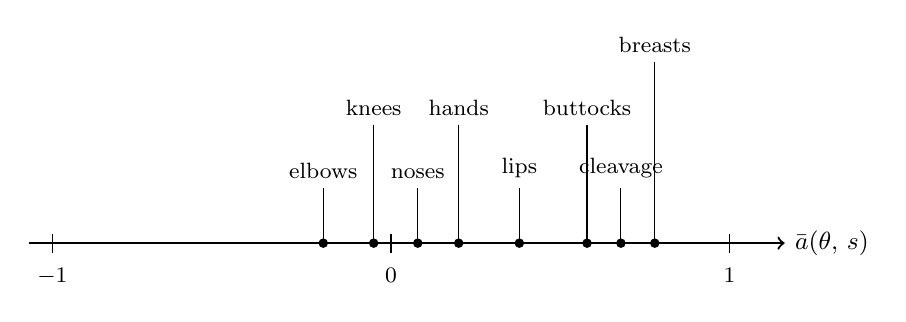
\begin{tikzpicture}[font=\footnotesize]
    % Scale: value v → x = 4.3v (fits within ~4.3in text width)
    % Range displayed: [-1, 1] → [-4.3, 4.3] cm

    % Number line
    \draw[thick, ->] (-4.6, 0) -- (5.0, 0)
      node[right, font=\small] {$\bar{a}(\theta,\, s)$};

    % Tick marks at -1, 0, 1
    \foreach \v/\lbl in {-4.3/{$-1$}, 0/{$0$}, 4.3/{$1$}} {
      \draw (\v, 0.12) -- (\v, -0.12) node[below=2pt] {\lbl};
    }

    % Each stimulus: dot on line + vertical stem + label at tip
    % Stems alternate short (0.7cm) and tall (1.5cm) for adjacent items
    % v * 4.3 = x position

    % elbows   v = -0.20 → x = -0.86,  stem h = 0.7
    \filldraw (-0.86, 0) circle (1.5pt);
    \draw[thin] (-0.86, 0) -- (-0.86, 0.7);
    \node[above] at (-0.86, 0.7) {elbows};

    % knees    v = -0.05 → x = -0.22,  stem h = 1.5
    \filldraw (-0.22, 0) circle (1.5pt);
    \draw[thin] (-0.22, 0) -- (-0.22, 1.5);
    \node[above] at (-0.22, 1.5) {knees};

    % noses    v =  0.08 → x =  0.34,  stem h = 0.7
    \filldraw (0.34, 0) circle (1.5pt);
    \draw[thin] (0.34, 0) -- (0.34, 0.7);
    \node[above] at (0.34, 0.7) {noses};

    % hands    v =  0.20 → x =  0.86,  stem h = 1.5
    \filldraw (0.86, 0) circle (1.5pt);
    \draw[thin] (0.86, 0) -- (0.86, 1.5);
    \node[above] at (0.86, 1.5) {hands};

    % lips     v =  0.38 → x =  1.63,  stem h = 0.7
    \filldraw (1.63, 0) circle (1.5pt);
    \draw[thin] (1.63, 0) -- (1.63, 0.7);
    \node[above] at (1.63, 0.7) {lips};

    % buttocks v =  0.58 → x =  2.49,  stem h = 1.5
    \filldraw (2.49, 0) circle (1.5pt);
    \draw[thin] (2.49, 0) -- (2.49, 1.5);
    \node[above] at (2.49, 1.5) {buttocks};

    % cleavage v =  0.68 → x =  2.92,  stem h = 0.7
    \filldraw (2.92, 0) circle (1.5pt);
    \draw[thin] (2.92, 0) -- (2.92, 0.7);
    \node[above] at (2.92, 0.7) {cleavage};

    % breasts  v =  0.78 → x =  3.35,  stem h = 2.3
    \filldraw (3.35, 0) circle (1.5pt);
    \draw[thin] (3.35, 0) -- (3.35, 2.3);
    \node[above] at (3.35, 2.3) {breasts};

  \end{tikzpicture}
  \caption{Approximate values of $\bar{a}(\{\textit{gender}=\text{men}\}, s)$ for selected stimuli $s$. Positions are illustrative, not empirically derived.}
  \label{fig:numberline}
\end{figure}
